\documentclass[../doc.tex]{subfiles}

\begin{document}

\section{Gameplay}

Chaque joueur se voit attribuer une cible et est cible d'un autre joueur.
Nous intégrons donc un système de sélection de cible, et un moyen pour le joueur de sélectionner un personnage (joueur ou non) à proximité de Lui

Nous avons également rajouté des objets pouvant être utilisé par les joueurs
(Echelles\footnote{Voir Figure 4}, Portes) et comptons en rajouter d'autres.
\begin{figure}[hbt!]
    \centering
    \begin{subfigure}[t]{0.3\textwidth}
        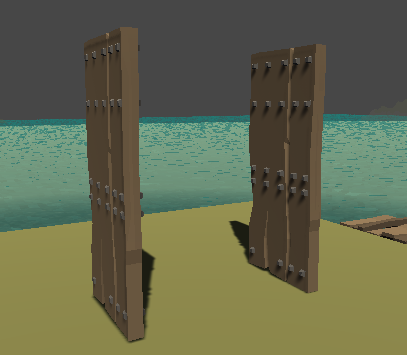
\includegraphics[scale=0.5]{doors_open.png} 
        \caption{Portes ouvertes}
    \end{subfigure}
    \hspace{50pt}
    \begin{subfigure}[t]{0.3\textwidth}
        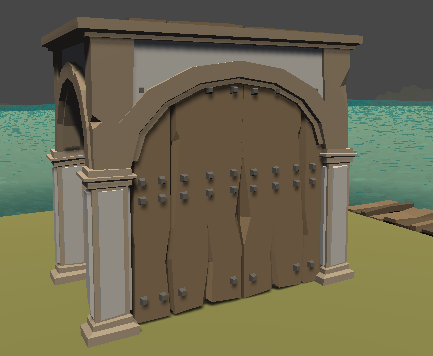
\includegraphics[scale=0.5]{doors_closed.png}
        \caption{Portes fermée avec arche}
    \end{subfigure}
    \caption{Exemple des portes que nous avons réalisé}
\end{figure}

\end{document}